\documentclass[a4paper]{article}

\usepackage[english, swedish]{babel}
\usepackage{float}
\usepackage[style=ieee]{biblatex}
\usepackage{csquotes}
\usepackage[toc,title]{appendix}
\usepackage{titlesec}
\usepackage{hyperref}

\hypersetup{
    colorlinks,
    citecolor=black,
    filecolor=black,
    linkcolor=black,
    urlcolor=black
}

\renewcommand\appendixtocname{Bilagor}


\addbibresource{references.bib}

\begin{document}
\pagenumbering{gobble}

\begin{titlepage}
    \centering

    \vspace*{0,5cm}

    \begin{LARGE}
        \textbf{Gymnasiearbete Handroid}
    \end{LARGE}

    \begin{Large}

        \vspace{1cm}

        Spårning och representation av fingerrörelser.

    \end{Large}

    \vspace{1cm}

    \begin{large}
        Gabriel Calota\\
        Jonathan Damsgaard Falck\\
        William Johansson
    \end{large}

    \vspace{0.5cm}
    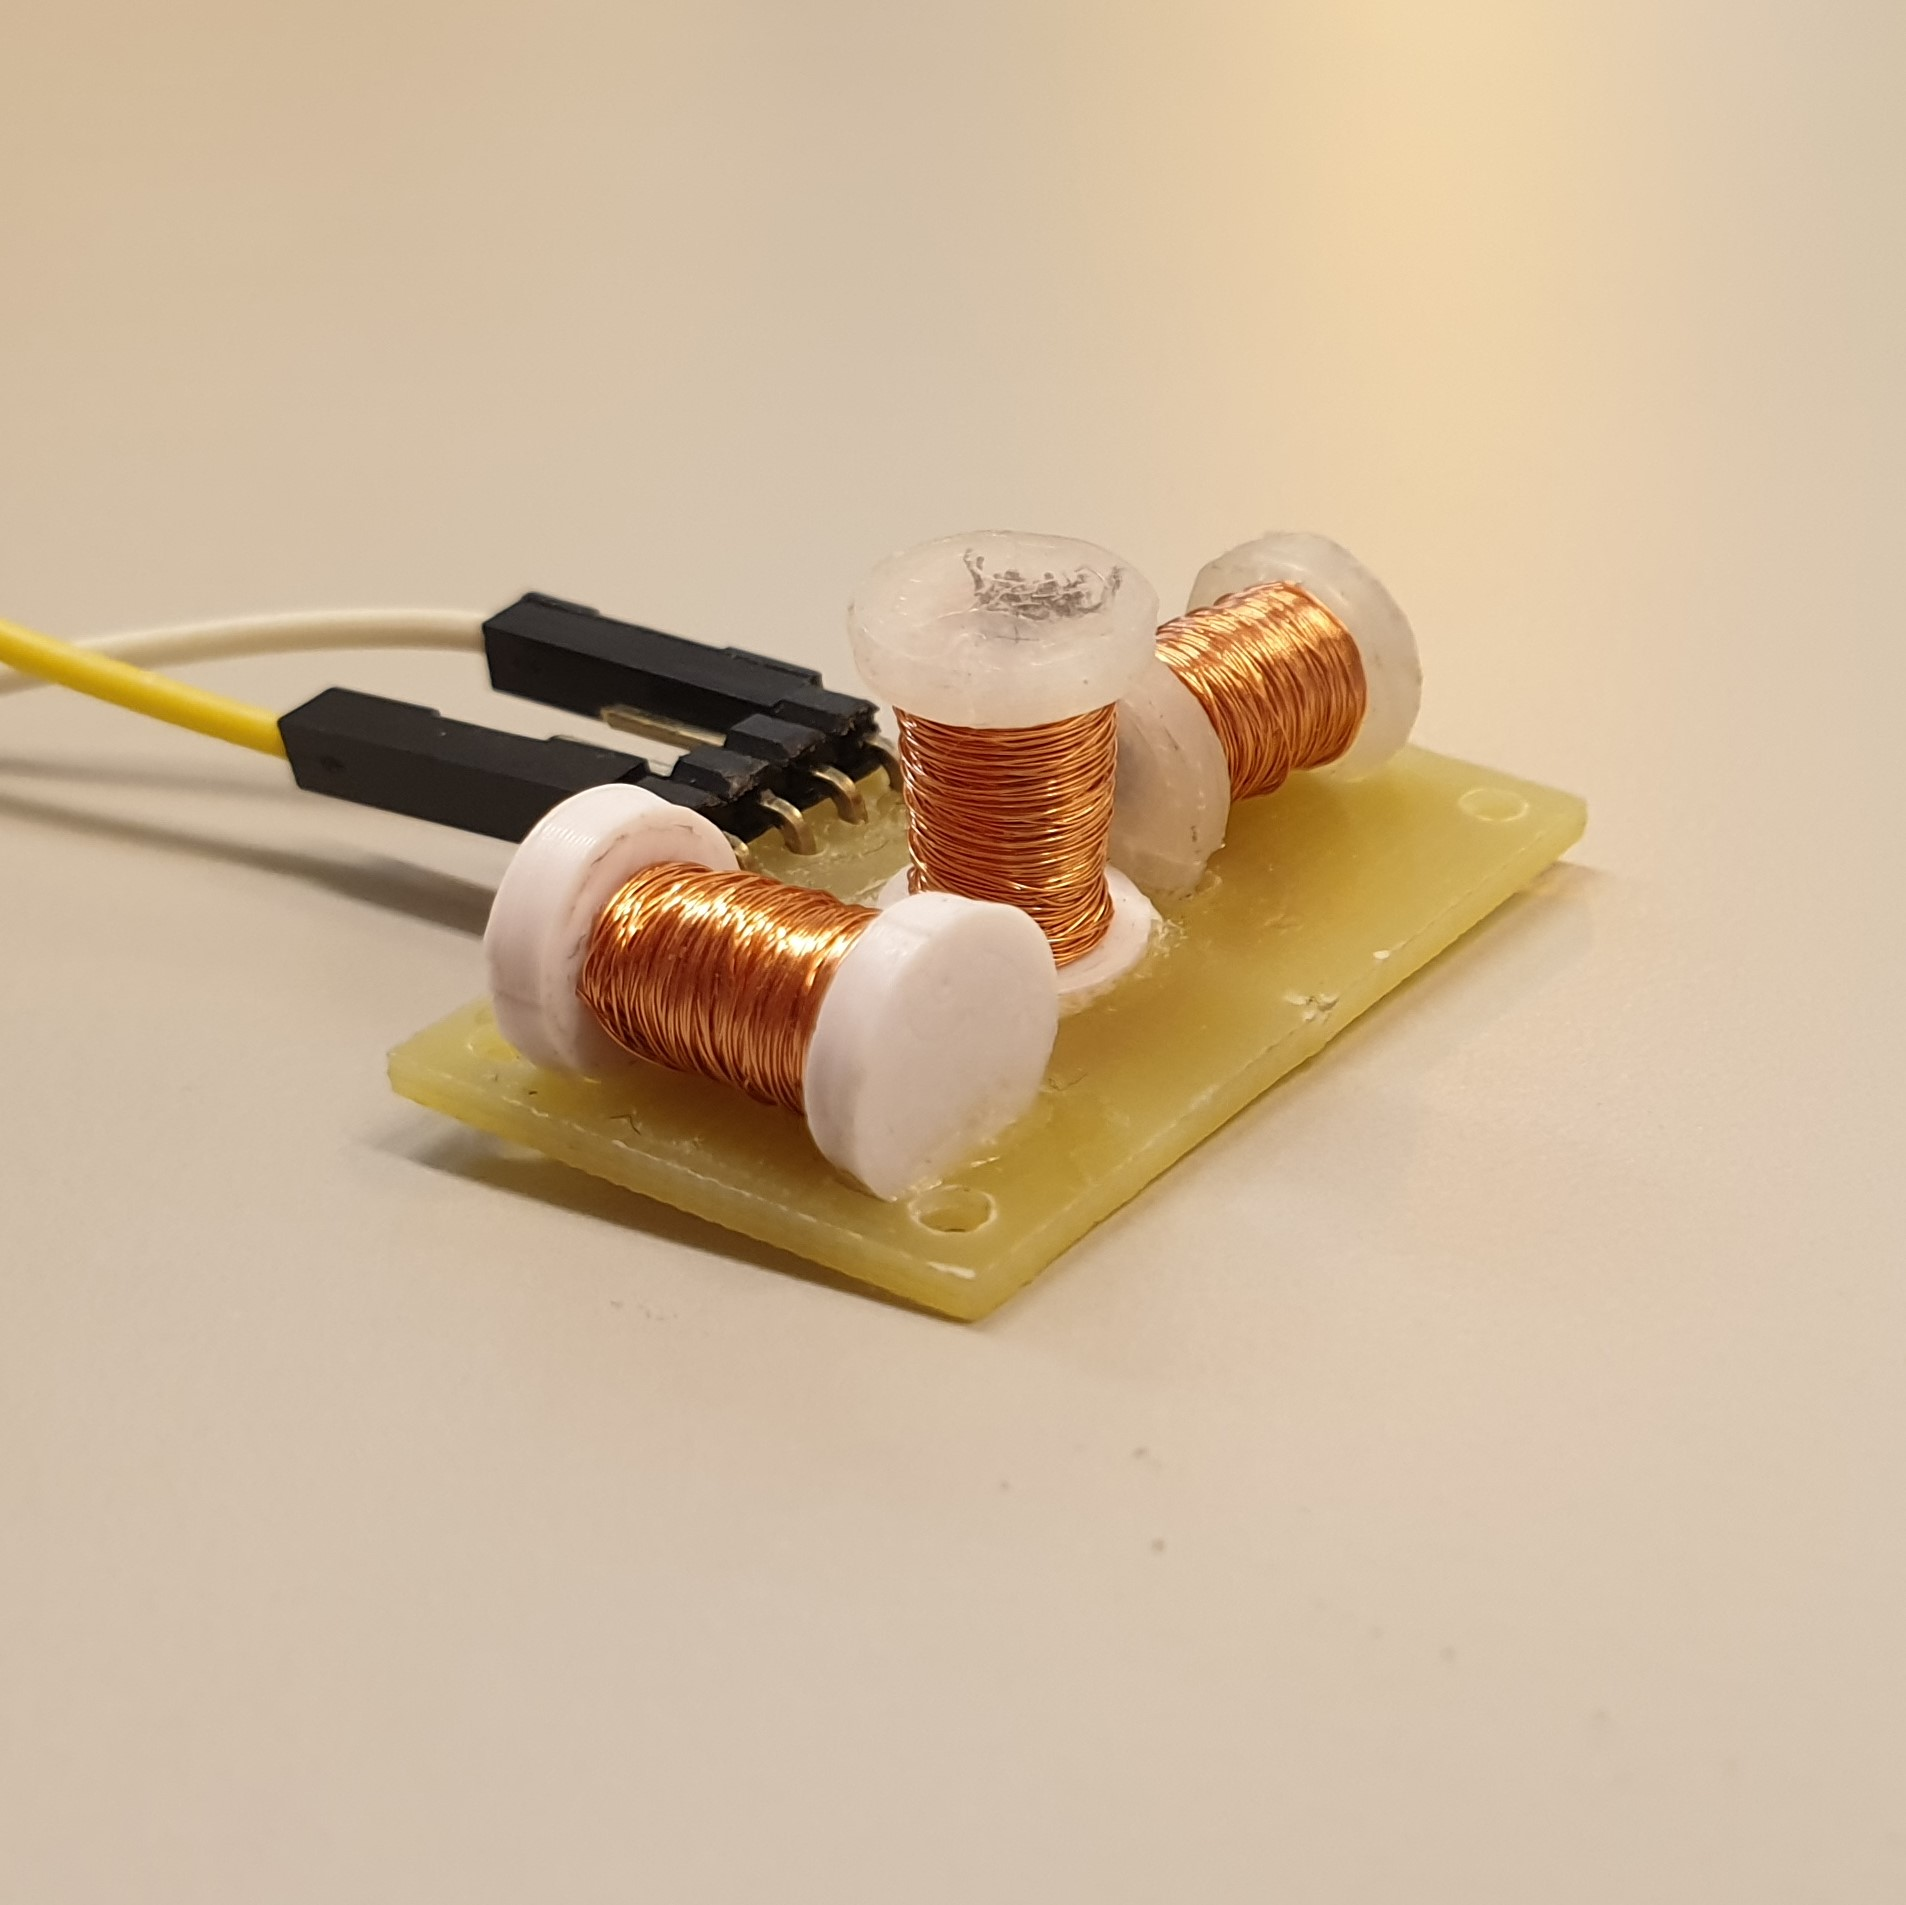
\includegraphics[width=\textwidth]{images/Spolhubb1.jpg}
    \vfill

    \begin{large}
        Lärosäte: ABB-Gymnasiet\\
        \vspace{0.5cm}
        Klass: 190S\\
        \vspace{0.5cm}
        Handledare: Andreas Jillram, ABB-Gymnasiet
    \end{large}

\end{titlepage}


\begin{abstract}

\end{abstract}

\begin{otherlanguage}{english}
    \begin{abstract}
    \end{abstract}
\end{otherlanguage}

\tableofcontents

\newpage
\pagenumbering{arabic}

\begin{sloppypar}

    \section{Inledning}
    \subsection{Syfte}
    Syftet med projektet är att undersöka hur människan finmotoriska rörelser kan detekteras, hur rörelserna såsom fingerrörelse kan användas som inmatning till olika system
    och utveckla ett prototyp som kan både detektera och återskapa fingerrörelser på en människohand.
    De finmotoriska rörelser kan återskapas antingen med en digital representation av rörelsen eller med en fysisk robothand.
    % De detekterade rörelserna ska sedan översättas till data som går att visualisera exempelvis genom att kontrollera en fysisk robothand eller digitalt i ett datorprogram.
    \subsection{Bakgrund}
    Det finns ett ökat intresse och en ökad efterfrågan på olika sätt för människan att interagera med datorer och robotar.
    Bland annat hur människokroppen kan användas för inmatning till datorprogram och till olika maskiner.
    Den här tekniken är som mest utvecklad inom virtual reality och augmented reality och det är inom dessa områden som tekniken i nuläget har störst användning.
    Tekniken är dock fortfarande relativt begränsad och använder mestadels grövre motorik som inmatning och förlorar den precision som kan ges av finmotoriska rörelser.

    % Vi ser ett ökande intresse för andra applikationer där människan agerar fjärrkontroll.   

    \subsection{Frågeställning}

    \section{Teori}
    För att få en bättre bild av hur en robothand kan skapas och styras med hjälp av olika sensorer undersöktes andra, liknande projekt.
    Projektet drog inspiration från en kandidatexamen från två KTH-studenter~\cite{KTHhand} med ett liknande syfte, och
    idéer för tummens funktion på den fysiska handen kom från ett projekt som hette \textit{Etho Hand}~\cite{EthoHand}
    vars syfte var att utveckla en hand som kunde utföra komplexa rörelser.


    \subsection{Elektromagnetism}
    \subsubsection{Magnetfält}
    Detta är elektromagnetism
    \subsubsection{Induktion}

    \subsection{Elektronik}
    \subsubsection{Spolar}
    \subsubsection{Kondensatorer}
    \subsubsection{Operationsförstärkare}
    \subsubsection{Filter}
    \subsubsection{Oscillatorer}
    \subsubsection{Flexsensorer}
    En flexsensor är en sensor som ändrar resistans proportionerligt med hur mycket den är böjd.
    Flexsensorer kan användas för att mätta gur mycket ett finger är böjd och de har använts i projekt och produkter som ... .
    \subsubsection{Accelerometer}
    \subsubsection{Mikrokontroller}

    \subsection{Bluetooth Low Energy}
    Bluetooth Low Energy liknar traditionell Bluetooth, men är mer energieffektiv.
    \subsubsection{Peripheral}
    \subsubsection{Central}

    \subsection{Rendering}
    \subsubsection{Unity}
    Unity är en programvara som möjliggör skapandet av real-time 3d-miljöer för spel, film etc. https://unity.com/our-company.

    \section{Metod och material}



    \subsection{Konstruktion}

    \subsubsection{3D-hand}
    En design för en fysisk 3D-hand skapades som skulle kontrolleras av fingerdetektionen.
    Designen bestod av servon som med hjälp av trådar styr fingrarna
    och 3d-modeler av fingersegment som kunde skrivas ut med en 3D-skrivare.

    \subsubsection{Spolar}
    \subsubsection{Montering på hand} %3d prints,  etc. bättre titel

    \subsection{Kretsar}
    \subsubsection{Filter}
    Filtret ska filtrera frekvenser som inte är inom ett visst frekvensområde och ett aktivt bandpassfilter valdes som filtertyp.
    Filterkretsen designades först med hjälp av formler för att bestämma värden på kondensatorer och resistorer.
    Kretsen testades sedan i simulering för att säkerställa att kretsens fungerar som förväntat,
    dock användes en ideal operationsförstärkare under simuleringen.
    När kretsen sedan simulerades med icke-ideal operationsförstärkare kunde kretsen inte längre filtrera signalen.
    Det visades sig att formlerna för kondensatorer och resistorer
    antog att operationsförstärkare var ideal för att kretsen skulle fungera.
    Kretsen designades sedan om med hjälp av ett filter designverktyg av Texas Instruments
    och fungerade i simulering med en icke-ideal operationsförstärkare.
    \subsubsection{Oscillator}


    \subsection{Rendering}
    \subsubsection{Mikrokontroller}
    Mikrokontrollen Arduino Nano 33 BLE används för att kommunicera med renderingsprogrammet.
    Mikrokontrollen väntar på renderingsprogrammet att ansluta och
    läser sedan av värdena från de olika sensorerna och publicerar dessa till en Bluetooth characteristics.
    För att åstadkomma kommunikation används biblioteket ArduinoBLE.

    \subsubsection{Renderingsprogram}
    Renderingsprogrammet som används är Unity.
    För att kommunicera med mikrokontrollen används BleWinrtDll och hand modellen kommer från Ultraleaps Unity Plugin.
    Programmet översätter värdena från sensorerna till rotationer i fingrarnas leder.





    \section{Resultat}
    \section{Diskussion och Slutsats}
    \subsection{Diskussion}

    \subsection{Slutsats}

    \section{Avslutning}




    \section{Källor}

    \appendices
    \titleformat{\section}[display]
    {\normalfont\Large\bfseries}{\appendixname\enspace\thesection}{.5em}{} %ny rad efter bilaga x
    \section{Renderingskod}

    \section{Oscillatorkrets}

    \section{Filterkrets}


\end{sloppypar}
\printbibliography[heading=none]

\end{document}